\begin{appendix}
    \chapter{Documentation d'un processus d'Altissia launcher}
    \label{ch:altissia-launcher-doc}
    
    \paragraph{}
    Altissia launcher contient environ soixante scripts.
    Certains processus nécessitent d'employer plusieurs de ces scripts et de procéder à certaines actions manuelles.
    
    \paragraph{}
    Il est donc nécessaire de documenter son utilisation.
    Nous utilisons Confluence, une application web pour créer collaborativement des documents, pour documenter les processus d'Altissia launcher.
    J'ai inclus ci-après les pages expliquant comment exporter les questions de test de niveau.
    
    \paragraph{}
    Le test de niveau est un test qui permet d'évaluer votre maîtrise d'une langue.
    Si vous le désirez, vous pouvez passer un test d'anglais gratuit sur \url{https://altissia.org/fr/test-niveau-anglais-gratuit/}.
    
    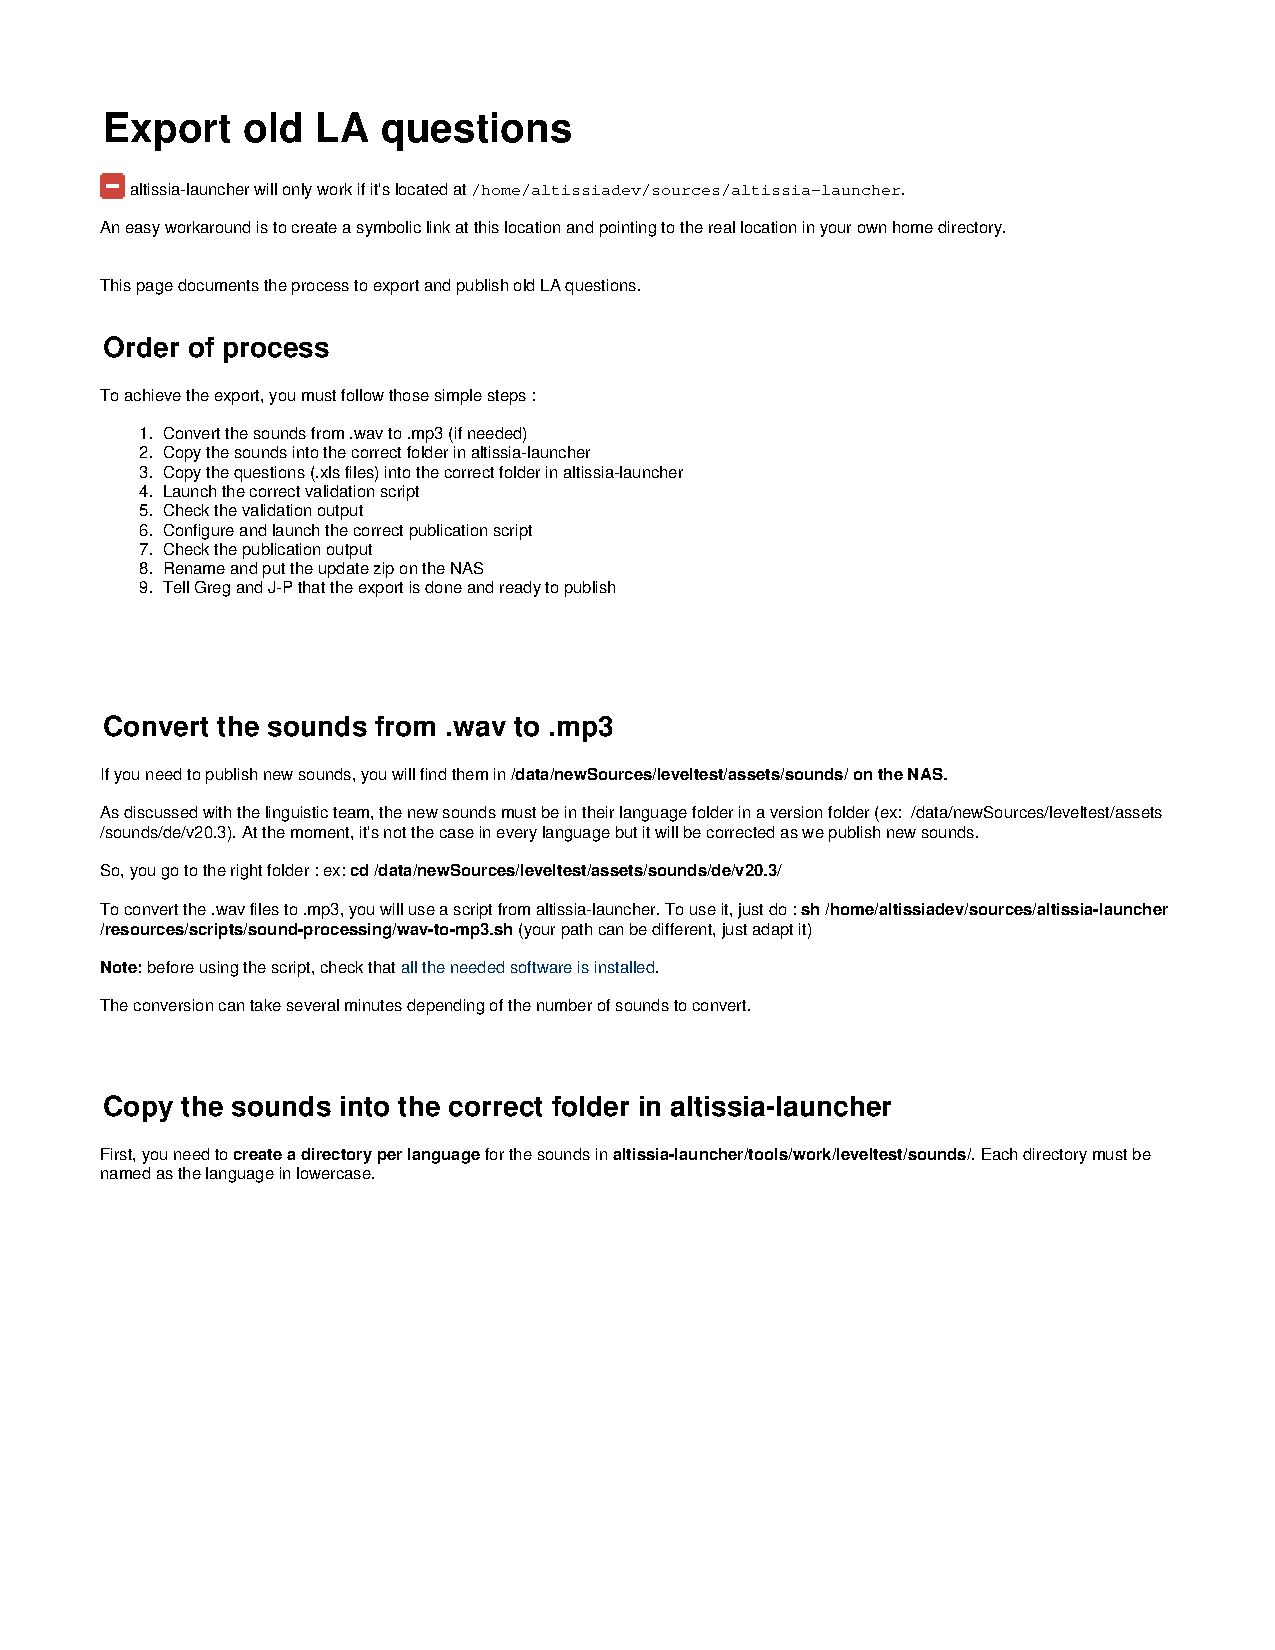
\includepdf[pages=-]{annexes/altissia-launcher-doc.pdf}
\end{appendix}